\documentclass[12pt,english]{article}
\usepackage{mathptmx}

\usepackage{color}
\usepackage[dvipsnames]{xcolor}
\definecolor{darkblue}{RGB}{0.,0.,139.}

\usepackage[top=1in, bottom=1in, left=1in, right=1in]{geometry}

\usepackage{amsmath}
\usepackage{amstext}
\usepackage{amssymb}
\usepackage{setspace}
\usepackage{lipsum}

\usepackage[authoryear]{natbib}
\usepackage{url}
\usepackage{booktabs}
\usepackage[flushleft]{threeparttable}
\usepackage{graphicx}
\usepackage{caption}
\usepackage{subcaption}
\usepackage[english]{babel}
\usepackage{pdflscape}
\usepackage[unicode=true,pdfusetitle,
 bookmarks=true,bookmarksnumbered=false,bookmarksopen=false,
 breaklinks=true,pdfborder={0 0 0},backref=false,
 colorlinks,citecolor=black,filecolor=black,
 linkcolor=black,urlcolor=black]
 {hyperref}
\usepackage[all]{hypcap} % Links point to top of image, builds on hyperref
\usepackage{breakurl}    % Allows urls to wrap, including hyperref

\linespread{2}

\begin{document}

\begin{singlespace}
\title{Tapping in to the potential of Craigslist data\thanks{Acknowledgements here, if any.}}
\end{singlespace}

\author{Karley Nadolski\thanks{Department of Economics, University of Oklahoma.\
E-mail~address:~\href{mailto:karley.j.nadolski@ou.edu}{karley.j.nadolski@ou.edu}}}

% \date{\today}
\date{May 4, 2020}

\maketitle

\begin{abstract}
\begin{singlespace}
Over the course of the last two decades, Craigslist has become one of the most popular websites on the internet. This website, devoted to classifieds-style advertisements, has the potential to be an invaluable data source for data scientists or economists looking to understand rental markets in the US at a faster pace and from a closer perspective. As webscraping becomes a more common skill set for those with a basic understanding of coding, the information on Craigslist becomes more accessible to data scientists at all levles. This paper will examine how Craigslist data has been used in the past and introduce a naive sentiment analysis project that charts the relationship between information provided by the author (captured in the length of the user-generated descriptions) of the rental listing and the price of the unit for rent (while holding constant several other variables of interest).  
\end{singlespace}

\end{abstract}
\vfill{}


\pagebreak{}


\section{Introduction}\label{sec:intro}

Craigslist was launched in 1995 as an email distribution service that featured local events in the San Francisco Bay Area. More than 25 years later, “craigslist” is now a household name, albeit a controversial one. An online forum for posting and viewing local classified advertisements, Craigslist is one of the most popular websites in the world. 

The site itself is organized into 497 subdomains (\citet{thompsongithub}), for each of the nearly 500 metropolitan areas that the website services. At a city level, users can find anything from job postings, to garage sales, to discussion boards, to personal ads that are all made available within a user-selected maximum geographic area. A user in Oklahoma City, Oklahoma could find short-term work in the “gigs” section of the website, while someone across town looks for a suitable vacation rental in the area. Although there are many features available for users on all Craigslist subdomains, the housing section of any subdomain is popular for both agents and renters. At any given time, a city’s Craigslist page will have thousands of apartment rental listings available for browsing. For prospective renters interested in getting a full glimpse of their options within a certain community, Craigslist provides a snapshot of available listings. For Economists interested in understanding rental markets at a local level in the US, Craigslist is also an invaluable source of the most up-to-date information.  

Even though Craigslist has potential to serve as an incomparable source of economic information, existing scholarship mainly focuses on Craigslist’s connection to fraudulent activity (\citet{Garg2013}) and the impact of crises too recent to be captured in more traditional data sources (like the COVID-19 pandemic) (\citet{Kuk2021}). There is room for more analysis to be done using the fine-grained data from Craigslist to supplement data sources like the Census or other commercial providers. As the housing market, and specifically the rental market within it, continues to operate online, social scientists should be using more advanced tools to create better and more effective data sets. Webscraping is an effective way to get information from Craigslist’s many subdomains in a more direct, automated way. This paper will use webscraping techniques within the R package “rvest” to scrape the Craigslist subdomain for apartment listings in Oklahoma City, Oklahoma. Using functions from the “SentimentAnalysis” package in R, this paper will seek to find relationships between Craigslist advertisements (their length, tone, and overall index of positivity, for example) and the price of rental listings in Oklahoma City with a minimum of 2 bedrooms, 1 bathroom, and 900 square feet.  

The main purpose of this paper is to gauge the effectiveness of using Craigslist data as a reliable source to examine the state of the rental market in Oklahoma City. Because of the breadth of unit-specific information available on Craigslist, it’s easy to collect and organize data that gives a glimpse of the OKC rental market from a more fine-grained perspective. Combining sentiment analysis with quantitative analysis, this paper will attempt to find and understand relationships between rental units (size, price, features) and how they are portrayed textually within the Craigslist platform). 

The rest of this paper is organized as follows: section 2 is the literature review will survey current literature about Craigslist, web scraping, and sentiment analysis, section 3 will introduce the Data and underline the web scraping process and cleaning needed to refine it, section 4 will outline empirical methods used for this analysis, section 5 will focus on the research findings, and section 6 will be devoted to the conclusion. 


\section{Literature Review}\label{sec:litreview}

In the sphere of economics, Craigslist has become an important resource for data scientists who want to better understand the rental housing market in different communities across the country. Traditional resources, like the Census Bureau’s American Community Survey or other commercial data sources, are not equipped to capture unit-to-unit information about rental listings or minute-to-minute updates as to the state of the rental market in given locations. The ACS often depends on a very small sample of American households to paint a picture of different consumer markets, so it is prone to inaccuracies (\citet{Boeing2017}). Tract-level data, which is often of the most interest to data scientists and public planners alike, only becomes available every 5 years. Associations of apartment managers, brokers, and other commercial sources focus primarily on large apartment complexes. With this information, it would be easy to miss the corners of the rental market devoted to garage apartments, condominiums or houses for rent,  or even small self-managed apartment buildings. Craigslist is better able to cover these gaps in available information because of how effectively the website has attracted users who post billions of Craigslist listings every day. 

Despite longstanding cultural attitudes and policy initiatives that incentivize homeownership, renting in the United States is incredibly important (\citet{Boeing2017}). Many young people are choosing to rent instead of buy. By 2013, 35\% of US households (amounting to about 43 million people) were renting their housing. Much of this activity takes place between private parties, without leaving a significant data trail of any kind. 

In the last two decades Craigslist became the dominant forum for information exchange in rental markets all across America, taking the place that the classified sections of print newspapers once held (\citet{Kuk2021}). Between 2000 and 2007 alone, Craigslist took \$5 billion in ad revenue from newspapers (\citet{Boeing2017}). By 2012, the revenue from classified ads dropped from \$20 billion (its highest level in 2000) to just \$4.6 billion—a decrease of 77\% (\citet{Johnson20}).  This complete transfer of market power, from print newspapers to websites, is a testament to how effective Craigslist is as an online bulletin board. Advertising costs are cut to nearly zero for all Craigslist users, advertisements reach a wider audience for a longer period of time, and the website’s interface allows users to search through listings in a personalized, convenient way (\citet{Fang2017}). Because of its simple, but effective model, Craigslist is the largest website for rental housing advertisements in the United States.

It’s important to mention that proprietary data from sources like Craigslist aren’t perfect representations of the larger rental market, but they are a valuable addition to more established data sources. Craigslist is a conduit for a vast array of user-generated data that flows through cities in real time. The market evolves at a quicker pace than what 5 year rolling averages can accurately capture, Craigslist can provide minute-by-minute updates that do a better job of encapsulating short-term trends in local conditions. Geoff Boeing and Paul Waddell used Craigslist data from across the country to study the nature of the Craigslist rental market. They found that “Real-time Craigslist data in particular fill a pressing need for planners to measure local-scale rental markets… to understand local conditions, advocate for realistic FMRs, and proactively address emerging affordability challenges” (\citet{Boeing2017}). The usefulness of data available on Craigslist can be attributed to the breadth of unit-specific information that each listing contains. 

All rental housing advertisements on Craigslist must contain advertised rent (although this number may differ from the negotiated amount that appears on the final lease agreement) and a textual description of the rental unit itself. The majority of advertisements also include an address or geocoded location, pictures of the unit, and specific information ranging from pet policy to square footage (\citet{Kuk2021}). Often times, users will advertise their rental listings on Craigslist multiple times to attract more attention as more listings are added to the page. These multiple listings will either be completely identical (with the same titles, descriptions, and basic unit information), or they will have different titles or descriptions to advertise the same unit. 

One way to analyze the significance of these textual descriptions is through sentiment analysis. Sentiment analysis is a computational study of people’s opinions, attitudes and emotions as conveyed through text (\citet{Medhat2014}). Often, sentiment analysis is done on customer reviews (which are often strongly opinionated in either a positive or a negative way). Computationally, sentiment analysis identifies the sentiment expressed in a document, a sentence, or an entity and then classifies its polarity (either qualitatively or quantitatively). Document-level analysis classifies the opinion that a document expresses by considering the whole document a basic information unit. Sentence-level analysis treats each sentence as its own basic information unit, or document. The first step to this analysis is identifying whether or not the basic unit (sentence or document) is objective or subjective. The second step is actually determining whether the basic unit is negative or positive. The other form of sentiment analysis, entity-level analysis, allows for different opinions about different aspects of the same entity. This level of sentiment analysis is more computationally intensive, but also allows for a much greater degree of detail in the analysis (\citet{Medhat2014}). Sentiment analysis has been used in many different areas of scholarship. Some scholars have, for example, integrated sentiment analysis into a commodity price forecast algorithm in order to increase forecast accuracy and reflect the relationships between the News and the price of sensitive commodities (\citet{Tseng2018})

This paper will primarily focus on document-level analysis concerning the user-written descriptions of rental listings on Craigslist and the sentence-level analysis of listing titles also written by the user. For text analysis to work, natural language processing and machine learning ideas and practices are combined to assign a sentiment score to a unit of text by referencing a sentiment library with manually scored adjectives and phrases. 

\section{Data}\label{sec:data}

The data used for this quantitative analysis was scraped from Craigslist’s subdomain for Oklahoma City, Oklahoma. The actual HTML parsing process was automated with the “rvest” package in R and its html\_node() function. The code builds a foundational search query that isolates Craigslist’s Oklahoma City subdomain’s apartment listings. Then it goes on to extract information about listing ID, listing title, monthly price of rental unit, the date that the posting was listed, the user-provided location of the unit, and the square footage for each listing. The code then goes on to examine each posted listing individually to scrape information about each unit’s longitudinal and latitudinal location and the textual description of the unit. After this code has been run, the data is collected into a data frame that includes information on every listing on the first page of the appropriate Craigslist page. To extract the listings on the subsequent pages, all of the above code is entered into a for loop that iteratively steps through each page of the query’s responses to collect all of the available data that fits the original query request. 

After the data has been scraped from Craigslist itself, it is ready to be cleaned and organized. Most of the data pulled from the website was formatted in the original code that did much of the scraping directly from Craigslist. There were some unreasonable rent observations (monthly rent of \$0 or \$50,000) that can reasonably be attributed to typos or formatting errors. These observations were deleted from the data set. The text descriptions from each individual listing required the most cleaning to remove punctuation and other superfluous characters that might get in the way of text analysis. Another big task while preparing the data was removing duplicate listings. As written earlier, users will sometimes choose to post their listing multiple times. Identical listings were trimmed so that only the first advertisement that appeared would remain in the data set. After the data was cleaned and appropriately trimmed, it was ready for analysis. 

The next step towards getting the data ready for quantitative analysis was performing sentiment analysis on both the descriptions for each listing and the title. The SentimentAnalysis package in R provides a few different easy routes to quickly measure the sentiment of written materials. The analyzeSentiment() function specifically took a vector of descriptions and returned information about the sentiment of each description (based on a few different pre-loaded dictionaries). The package automatically references a few different sentiment dictionaries, including Harvard-IV (GI), Henry’s Financial (HE), and Loughran-McDonald Financial (LM) dictionaries. The package also heavily references the sentiment dictionary (key.pol) within the “qdap” package in R. 

The analyzeSentiment() function takes in a vector of basic information units and delivers a data frame that summarizes the sentiment analysis with 17 unique metrics. Each dictionary (GI, HE, LM, and QDAP) has its own assessment, and numeration, of the sentiment of each description and title.  The function also automatically counts the number of words in each text-based observation. After the sentiment analysis is finished, the results from it were added to the original dataset to be used for linear regression. 

As a final step before linear regression, it’s worthwhile to look at the relationship between different variables and the price of the rental unit. These relationships can then be used to decide which variables to include within the final regression model. 


This 1200-unit snapshot of the rental market for units with 2 bedrooms, 1 bathroom, and a minimum of 900 square feet provides a valuable peek into the Oklahoma City rental market. Geographically, the units are spread out from Edmond to Norman (with a single unit located as far west as Elk City). A map of the listings within the Oklahoma City Metro area is displayed in Figure \ref{fig:fig1} 

Within the sample, the median monthly rent was \$1,050 and the median square footage was 1,152 ft2. The highest rent per unit, after cleaning, is \$5,300 and the lowest rent per unit is \$175 per month. Similar quantitative analysis projects that review rental markets in certain regions of the country use rent by square foot as an important metric for comparison across markets. In Oklahoma City, the mean rent by square foot is \$0.895 and the median is \$0.918. Performing naïve sentiment analysis showed that each unit’s unique description ranged in length from 2 to 385 words. Figure \ref{fig:fig2} contains plots depicting each relationship graphically. 
 

Table \ref{tab:descriptives} contains summary statistics.


\section{Empirical Methods}\label{sec:methods}

Rental prices are affected by many factors that concern the rental unit itself as well as its location and amenities. Many Craigslist listings include information about all of these contributing factors. Often, users will use the description as a place to describe the characteristics of the listing that aren’t as easily quantified. These characteristics might include the rental unit’s pet policy, the amenities included in the lease agreement, the attractions of the surrounding area, or even special promotions like signing bonuses or deals on rent payments. This paper will create a linear regression model that attempts to characterize the relationship between the price of a rental unit and its Craigslist description while holding constant more easily quantifiable characteristics like square footage or the number of bedrooms. 

It’s clear that the strongest correlative relationship between two variables in the Craigslist dataset is between the price of each rental unit and its square footage. When other factors are held constant, it is common sense that price would mainly be affected by the square footage of each particular rental unit. Because the relationship between price and metrics of sentiment analysis can reasonably be expected to be weaker in comparison, square footage will be used as a control variable. The other control variable in this model is the number of bedrooms in each rental unit. All of these apartments in this data set have at least 2 full bedrooms, but some listings have as many as 5. In addition to square footage and number of bedrooms, the regression model will also include a measure of the overall positive sentiment of the description (p.QDAP), the number of words used in the description (wordcount), the number of words used in the title (t.wordcount), and the overall direction of the sentiment in the title itself (t.direction). While this approach does explore a number of different methods, the primary empirical model can be depicted in the following equation:

\begin{equation}
\label{eq:1}
Y_{price}=\beta_{0} + \beta_{1}X_{sqft} + \beta_{2} X_{bdrms} + \beta_{3}X_{p.QDAP} + \beta_{4}X_{wordcount} + \beta_{5}X_{t.wordcount}+\beta_{6}X_{t.direction} + \varepsilon,
\end{equation}
where $Y_{price}$ is a continuous variable describing the price of each rental listing, $X_{sqft}$ is the square footage of the rental unit, $X_{bdrms}$ is the number of bedrooms, $X_{p.QDAP}$ is the positivity index from the listing's description, $X_{wordcount}$ and $X_{t.wordcount}$ are the word counts for the description and the title, respectively, and finally $X_{t.direction}$ describes the sentiment of the listing title. This regression is done in R, using the lm() function from R’s base package. A second robust regression was done using the rlm() function from the “MASS” package to correct for possible heteroskedasticity. The results of the regression will be displayed and interpreted in the following section.

\section{Research Findings}\label{sec:results}

The results of this simple linear regression were not surprising, but they did provide an interesting insight into the premium of information in online classified-style advertising. The main results are reported in Table \ref{tab:estimates}.

As was expected, the most significant regression coefficients are sqft and bdrms with predicted values of 0.896 and -236.32 respectively. The negative sign on the coefficient for bdrms only appears when sqft is also included as a control variable within the model. This shows the relationship between price and number of bedrooms when square footage is held equal. The positive relationship between bdrms and price seen when sqft is not included in the model is captured more effectively by the benefit of an extra square foot of space when both variables are used as controls in a model. 

In a less expected way, the only other coefficient with a p-score less than 2x10-16 is the word count of the description. This BETA HAT estimate of 1.885 shows that for every additional word in the description, the price rises by about \$2 per month. It would be unreasonable to assume causality based on this simple regression, but it does show an interesting premium that information has within the Craigslist marketplace. Advertisements that are longer, usually include more information about the unit being advertised. This extra information is important for potential renters who are interested in knowing more about the unit than just the bare minimum that Craigslist requires. The word count for the title also has a statistically significant relationship with price from this model, but this particular relationship is negative (with a BETA HAT estimate of -12.58). This might relate to a salesman-like strategy among Craigslist users who prefer snappy titles and longer, more informative descriptions. 

The other variable in this regression deals with the overall sentiment of the title of each individual listing. Both the neutral and the positive directionality of the sentiment in the listing title are positively related to the price, with a larger premium on explicitly positive titles. The p-value for each of these dummy variables is between 0.05 and 0.01. This estimation, along with the evaluation of title word count, shows that listings with short but explicitly positive titles do slightly better than neutral ones. 

The final variable in this regression deals with the positivity of each listing’s description. The model shows a non-significant positive relationship between p.QDAP and price. Classified ads are often explicitly positive, making it difficult to find the true value of a positive description. 

\section{Conclusion}\label{sec:conclusion}

In Oklahoma City, like in many cities across the United States, there exists a rental market that Craigslist is uniquely able to summarize. Traditional data sources that cover rental markets in the United States aren’t able to release data at a fast enough pace to accurately characterize the market as it changes. With an introductory knowledge of webscraping, it’s possible to analyze data from a local Craigslist subdomain in real time. As housing markets and the internet grow and change together, it’s important that data scientists are prepared to take advantage of new and changing data sources. 

This project used webscraping techniques, from the “rvest” package in R, and sentiment analysis tools, from the SentimentAnalysis package, to analyze a corner of the rental market in Oklahoma City. After using linear regression to model the relationship between square footage, number of bedrooms, length of unit description, positivity of unit description, length of listing title,  and the sentiment direction of the listing title, some patterns became clear. Longer descriptions often meant that a listing would have a higher rental price (about \$2 per word, all else equal), while longer titles meant that the rental price would be lower. Sentiment analysis showed that most descriptions on Craigslist are slightly positive in sentiment, and that extra positivity isn’t significantly correlated with higher rental prices. 

The preliminary findings in this project leave room for more questions to be asked. Questions like: Why do longer descriptions often coincide with higher rental rates? Is it because longer descriptions reflect the number of amenities available to renters or is it a matter of transparency between agent and prospective renter? Or how does this Oklahoma City specific information relate to information on a national level? Tapping into the wealth of information on Craigslist could be a good first step in answering these questions.


\vfill
\pagebreak{}
\begin{spacing}{1.0}
\bibliographystyle{jpe}
\bibliography{References.bib}
\addcontentsline{toc}{section}{References}
\end{spacing}

\vfill
\pagebreak{}
\clearpage

%========================================
% FIGURES AND TABLES 
%========================================
\section*{Figures and Tables}\label{sec:figTables}
\addcontentsline{toc}{section}{Figures and Tables}
%----------------------------------------
% Figure 1
%----------------------------------------
\begin{figure} [ht]
\centering
\begin{subfigure}{.5\textwidth}
  \centering
  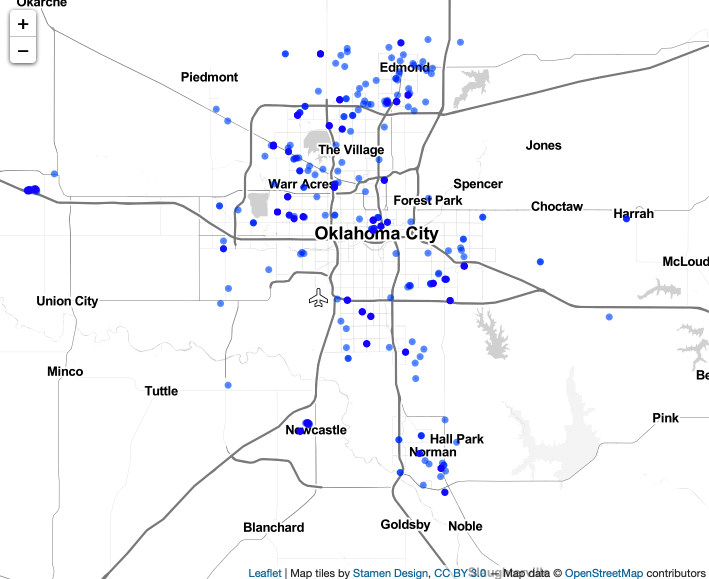
\includegraphics[width=.8\linewidth]{craigslist.mapfar.png}
  \caption{Larger Oklahoma City Area}
  \label{fig:sub1}
\end{subfigure}%
\begin{subfigure}{.5\textwidth}
  \centering
  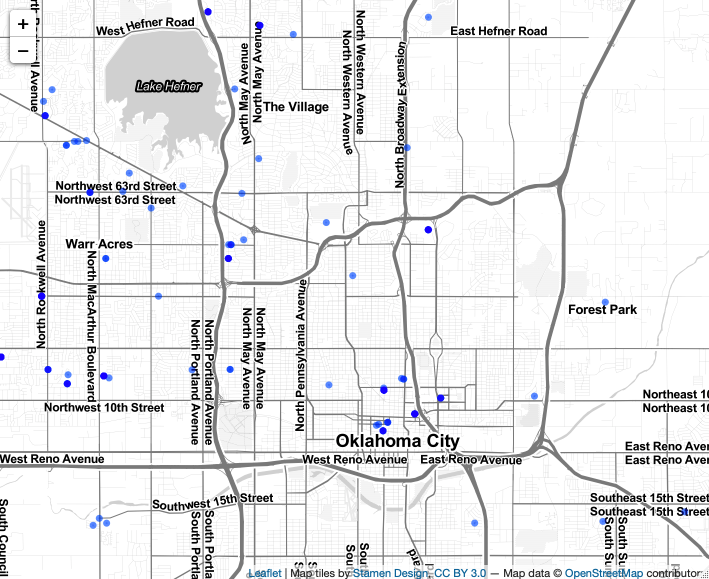
\includegraphics[width=.8\linewidth]{craigslist.mapclose.png}
  \caption{Close-up of Oklahoma City Neighborhoods}
  \label{fig:sub2}
\end{subfigure}
\caption{Map of Oklahoma City Metro Area with Craigslist Listings displayed Geographically}
\label{fig:fig1}
\end{figure}

%----------------------------------------
% Figure 2
%----------------------------------------
\begin{figure}[ht]
\centering
\bigskip{}
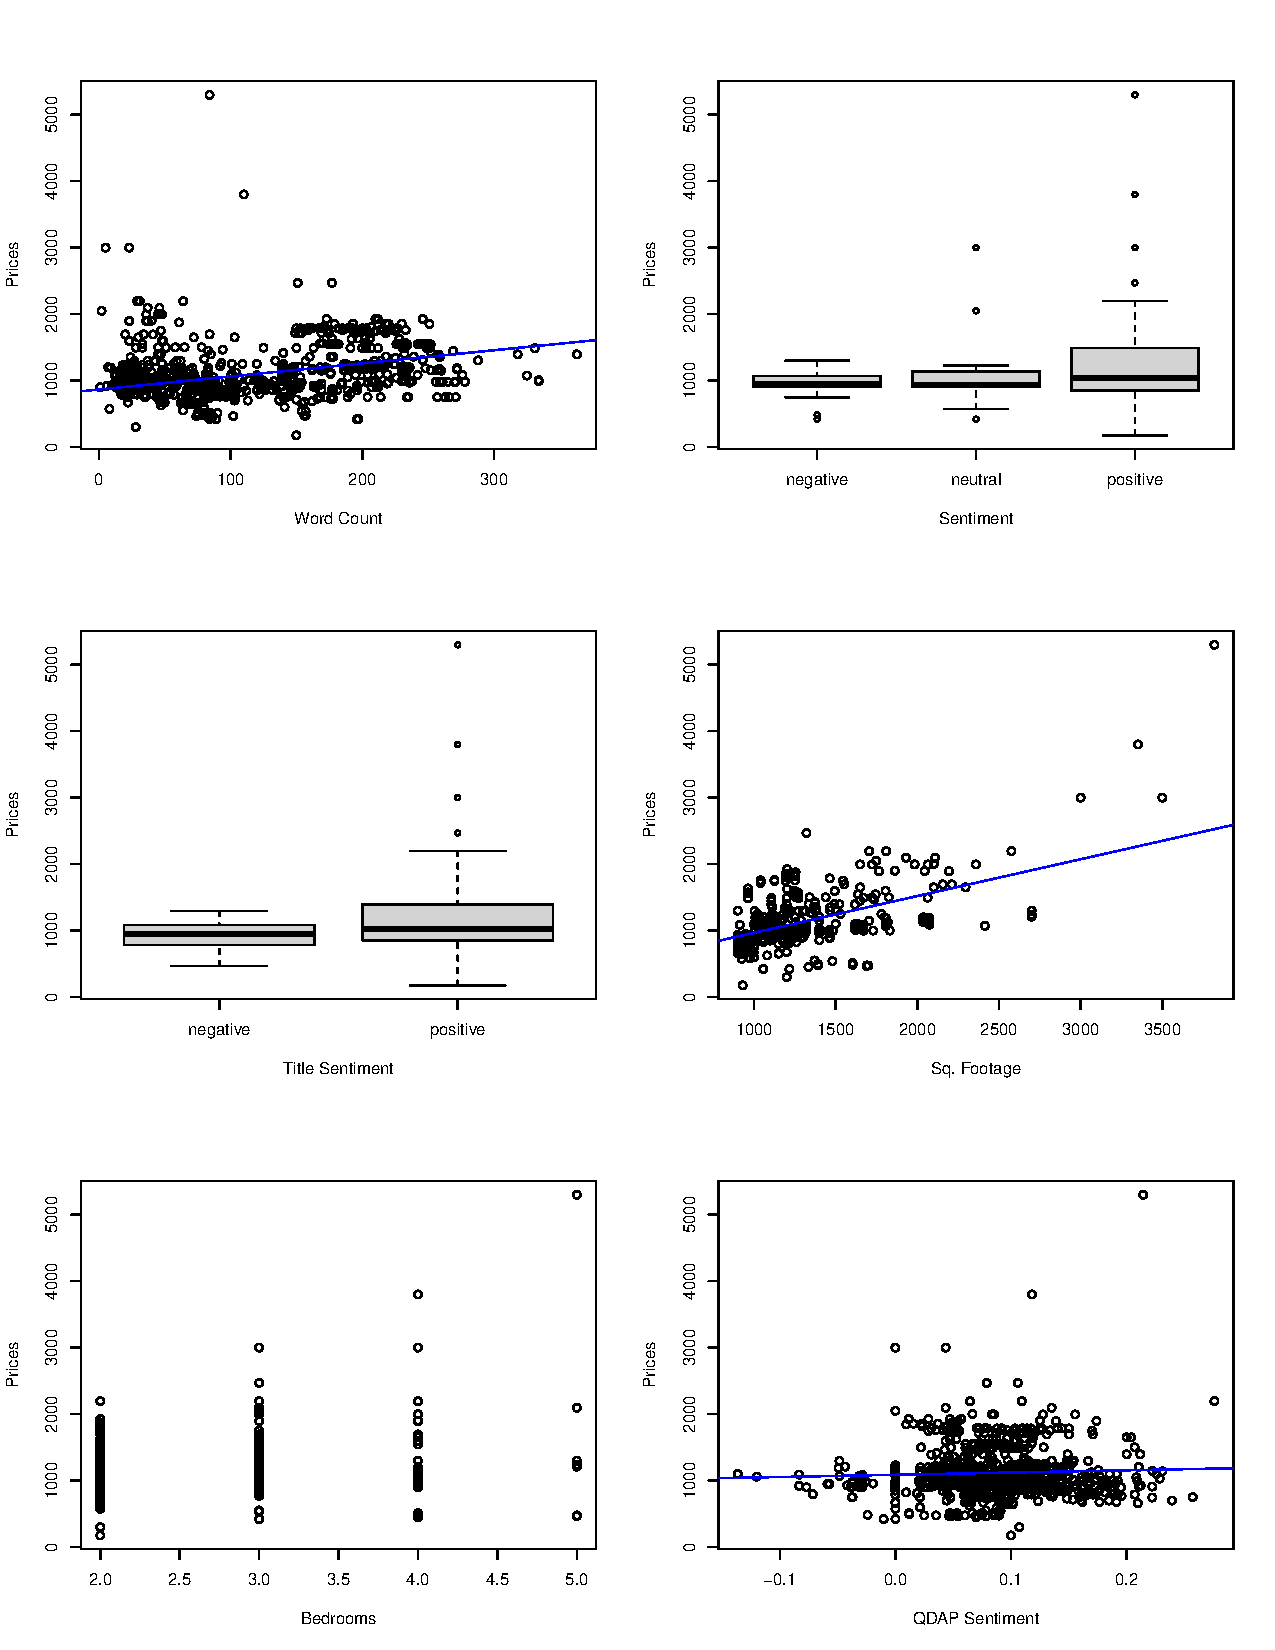
\includegraphics[width=.9\linewidth]{craigslist.plots.pdf}
\caption{Relationships between different explanatory variables and Unit Price}
\label{fig:fig2}
\end{figure}


%----------------------------------------
% Table 1
%----------------------------------------

\begin{table}[ht]
\caption{OLS estimates}
\label{tab:estimates} 
\centering
\begin{threeparttable}
\begin{tabular}{lccc}
\toprule
                            & Estimate    & Std. Error & P-value \\
\midrule
sqft        & 0.89505***   & (0.03317)    & $<2e-16$    \\
bdrms  & -234.539***   & (18.02865)   & $<2e-16$ \\
p.QDAP        &      229.54856 & (184.04089)  & 0.21255 \\
wordcount     &    1.87407***  & (0.10400)    & $<2e-16$\\
t.wordcount & -12.57888**  & (4.26128) & 0.00322 \\
t.directionneutral & 86.17754* & (41.89659) & 0.03992 \\
t.directionpositive & 100.19908* & (41.44415) & 0.01577 \\
\bottomrule
\end{tabular}
\footnotesize Notes: Standard errors in parentheses. ***Significantly different from zero at the .1\% level; **Significantly different from zero at the 1\% level. *Significantly different from zero at the 5\% level. 
\end{threeparttable}
\end{table}


\end{document}
